\documentclass[10pt,final,a4paper,oneside,onecolumn]{article}

%%==========================================================================
%% Packages
%%==========================================================================
\usepackage[a4paper,left=3.5cm,right=3.5cm,top=3cm,bottom=3cm]{geometry} %% change page layout; remove for IEEE paper format
\usepackage[T1]{fontenc}                        %% output font encoding for international characters (e.g., accented)
\usepackage[cmex10]{amsmath}                    %% math typesetting; consider using the [cmex10] option
\usepackage{amssymb}                            %% special (symbol) fonts for math typesetting
\usepackage{amsthm}                             %% theorem styles
\usepackage{dsfont}                             %% double stroke roman fonts: the real numbers R: $\mathds{R}$
\usepackage{mathrsfs}                           %% formal script fonts: the Laplace transform L: $\mathscr{L}$
\usepackage[pdftex]{graphicx}                   %% graphics control; use dvips for TeXify; use pdftex for PDFTeXify
\usepackage{array}                              %% array functionality (array, tabular)
\usepackage{upgreek}                            %% upright Greek letters; add the prefix 'up', e.g. \upphi
\usepackage{stfloats}                           %% improved handling of floats
\usepackage{multirow}                           %% cells spanning multiple rows in tables
%\usepackage{subfigure}                         %% subfigures and corresponding captions (for use with IEEEconf.cls)
\usepackage{subfig}                             %% subfigures (IEEEtran.cls: set caption=false)
\usepackage{fancyhdr}                           %% page headers and footers
\usepackage[official,left]{eurosym}             %% the euro symbol; command: \euro
\usepackage{appendix}                           %% appendix layout
\usepackage{xspace}                             %% add space after macro depending on context
\usepackage{verbatim}                           %% provides the comment environment
\usepackage[dutch,USenglish]{babel}             %% language support
\usepackage{wrapfig}                            %% wrapping text around figures
\usepackage{longtable}                          %% tables spanning multiple pages
\usepackage{pgfplots}                           %% support for TikZ figures (Matlab/Python)
\pgfplotsset{compat=1.14}						%% Run in backwards compatibility mode
\usepackage[breaklinks=true,hidelinks,          %% implement hyperlinks (dvips yields minor problems with breaklinks;
bookmarksnumbered=true]{hyperref}   %% IEEEtran: set bookmarks=false)
%\usepackage[hyphenbreaks]{breakurl}            %% allow line breaks in URLs (don't use with PDFTeX)
\usepackage[final]{pdfpages}                    %% Include other pdfs
\usepackage[capitalize]{cleveref}				%% Referensing to figures, equations, etc.
\usepackage{units}								%% Appropriate behavior of units
\usepackage[utf8]{inputenc}   				 	%% utf8 support (required for biblatex)
\usepackage{csquotes}							%% Quoted texts are typeset according to rules of main language
\usepackage[style=ieee,doi=false,isbn=false,url=false,date=year,minbibnames=15,maxbibnames=15,backend=biber]{biblatex}
%\renewcommand*{\bibfont}{\footnotesize}		%% Use this for papers
\setlength{\biblabelsep}{\labelsep}
\bibliography{../../bib}

%%==========================================================================
%% Define reference stuff
%%==========================================================================
\crefname{figure}{Figure}{Figures}
\crefname{equation}{}{}

%%==========================================================================
%% Define header/title stuff
%%==========================================================================
\newcommand{\progressreportnumber}{35}
\renewcommand{\author}{Erwin de Gelder}
\renewcommand{\date}{December 17, 2020}
\renewcommand{\title}{Performance assessment of automated vehicles using real-world driving scenarios}

%%==========================================================================
%% Fancy headers and footers
%%==========================================================================
\pagestyle{fancy}                                       %% set page style
\fancyhf{}                                              %% clear all header & footer fields
\fancyhead[L]{Progress report \progressreportnumber}    %% define headers (LE: left field/even pages, etc.)
\fancyhead[R]{\author, \date}                           %% similar
\fancyfoot[C]{\thepage}                                 %% define footer

\begin{document}
	
\begin{center}
	\begin{tabular}{c}
		\title \\ \\
		\textbf{\huge Progress report \progressreportnumber} \\ \\
		\author \\ 
		\date
	\end{tabular}
\end{center}

\section{Previous meeting minutes}

\begin{itemize}
	\item We did a yearly progress review. No big concerns were raised. I have sent the yearly progress report to Mascha Toppenberg and she forwarded it to the DMA system.
\end{itemize}

\section{Summary of work}

\begin{itemize}
	\item I enrolled for few graduate school courses in order to obtain the final GS credits I need (I need 3.5 more credits). I enrolled for the following courses:
	\begin{itemize}
		\item 2 GS credits: Effective Negotiation: Win-Win Communication;
		\item 1 GS credit: Time Management - Individual Crash Course; and
		\item 1 GS credit: Career Development - Personal Branding, Presenting Yourself Effectively.
	\end{itemize}
	
	\item I worked on the method for generating test scenarios.
	 I think I have enough material for an article. 
	 The results for the case study look good. 
	 In the article, I want to address two main topics. 
	 The first topic is a new approach for generating the test scenarios. 
	 The second topic is a new metric for evaluating the set of generated test scenarios. 
	 This latter topic still needs some work. 
	 I want to do few more experiments before starting to write the article.
	 I do this work together with Jan-Pieter, Jasper Hof (former student), and Eric Cator (prof  Applied Stochastics at RU Nijmegen) and I will discuss the results with the experiments with them first.
	 
	 \item I continued my work regarding the risk quantification. 
	 Two meetings ago (October 8), I mentioned that in the case study, I obtained extremely low probabilities of collisions (in the order of $10^{-10}$). 
	 As a result, I think we can go into two different directions for this research:
	 \begin{enumerate}
		 \item Propose a method for doing the importance sampling, such that the very low probabilities can still be estimated with reasonable accuracy.
		 \item Complement the scenarios with certain events, such as poor weather conditions or poor road conditions, such that the probabilities of collisions become higher.
	 \end{enumerate}
	 I chose to go for the second direction.
	 The main reason is that it better suits the needs of the industry, because of the upcoming standardization regarding the Safety Of The Intended Functionality (SOTIF) \cite{ISO21448}.
	 For SOTIF, there is a need to evaluate risks such as driving in poor weather conditions or with poor road conditions (e.g., low friction).
	 I am still working on the simulations, but I have good hope that after a few weeks, I can start writing.
	 In the case study, I want to look at the following events/conditions and scenarios:
	 \begin{itemize}
		 \item The event of having ``false positives'', e.g., detecting an object on the road while in reality there is no object. This could happen when passing through an underpass. This is mainly a risk for the car driving behind the automated vehicle.
		 \item The event of having ``false negatives'', e.g., not detecting an object on the road while in reality there is an object. The simulations will focus on the ability of the driver to take over and to prevent a collision.
		 \item The condition of having a low road friction and, thus, a limited braking capacity, in combination with scenarios ``lead vehicle decelerating'', ``approaching slower vehicle'', ``cut-in of other vehicle in front'', ``cut-out of vehicle in front while having another vehicle in front''.
		 \item The condition of driving on a graded road in combination with the aforementioned scenarios.
	 \end{itemize}
	 
	 \item For a TNO project, I have been working on a metric that can be used real time (e.g., on a vehicle while driving in real traffic) for evaluating the risk at each moment in time.
	 I proposed a metric for this which is a generalization of the metric presented by \autocite{wang2014evaluation}.
	 That is, with a certain configuration, my proposed metric produces the same result as the metric proposed by \textcite{wang2014evaluation}.
	 In this TNO project, we decided to publish this metric. 
	 Therefore, I started writing a paper on this topic.
	 My proposal is to aim for a journal article. 
	 A possible journal could be Accident Analysis \& Prevention (same as \autocite{wang2014evaluation}).
	 Alternatively, we could aim for the special issue ``Traffic Modelling and Control for Smart, Safe and Green Mobility'' in \emph{IEEE Open Journal of Intelligent Transportation Systems} (deadline: April 30, 2021).
\end{itemize}

\section{Future plans}

In \cref{fig:planning}, the updated planning is shown. There are a few changes compared to the latest planning (see \cref{fig:old planning}):
\begin{itemize}
	\item The ontology article has been submitted to IEEE Transactions on Intelligent Vehicles as opposed to IEEE Access. 
	If the article will be rejected, we might submit it to IEEE Access.
	
	\item A row is added with the article I want to write on a ``surrogate safety metric''. This is mentioned in the last item under \emph{summary of work}.
\end{itemize}

\begin{figure}[t]
	\centering
	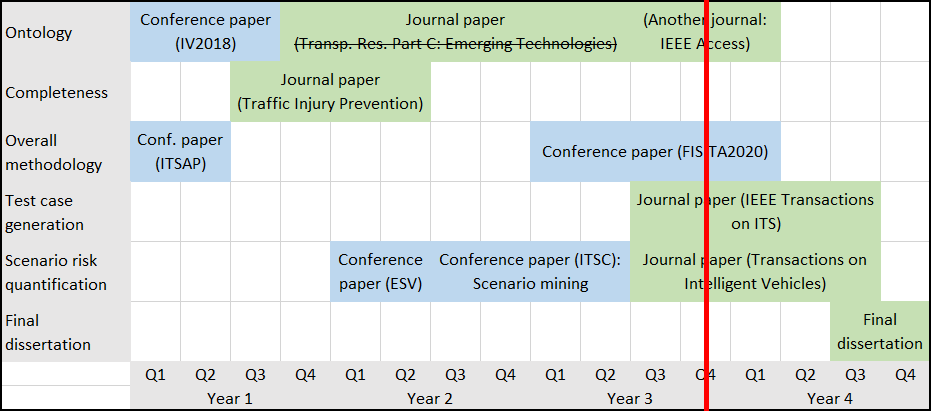
\includegraphics[width=\linewidth]{planning.png}
	\caption{Planning as proposed during the progress meeting on August 12. Note the differences with the updated planning shown in \cref{fig:planning}.}
	\label{fig:old planning}
\end{figure}

\begin{figure}[t]
	\centering
	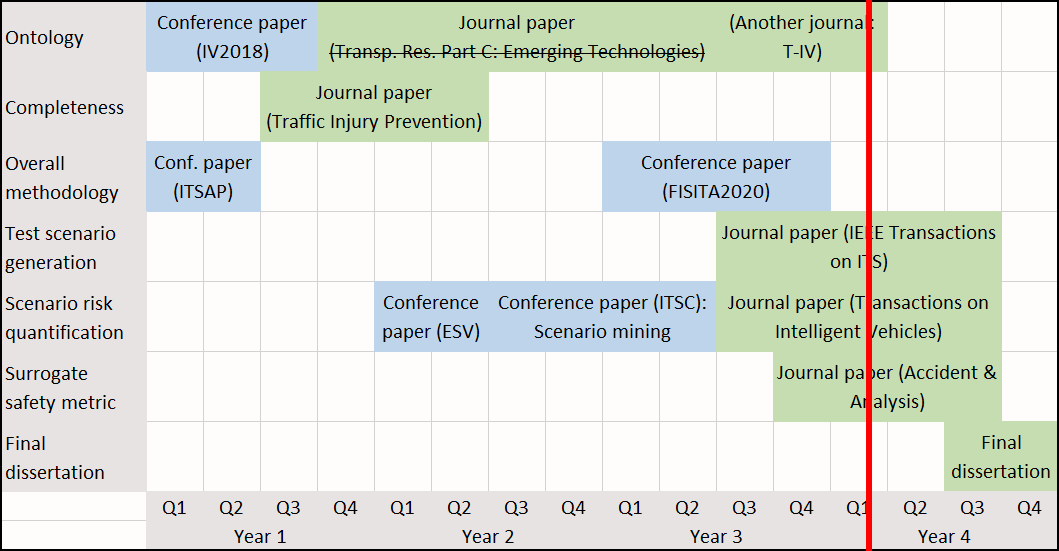
\includegraphics[width=\linewidth]{new_planning.png}
	\caption{Proposed planning at the time of this report. The red line indicated the time when writing this report.}
	\label{fig:planning}
\end{figure}

For the coming weeks, I want to focus on the following:
\begin{itemize}
	\item Finish first draft on the \textit{surrogate safety metric}.
	\item Finish the simulations for the risk quantification.
	\item Start with writing for the article on test scenario generation.
\end{itemize}



\printbibliography

%\clearpage
%\includepdf[pages=-,pagecommand={},width=\paperwidth]{../../""/.pdf}

\end{document}